\documentclass[11pt]{article}
\usepackage[a4paper,margin=1in]{geometry}
\usepackage{amsmath,amssymb,amsthm}
\usepackage{tikz}
\usepackage{xcolor}
\usepackage{booktabs}
\usepackage[hidelinks]{hyperref}
\hypersetup{pdftitle={Every number except three},pdfauthor={Vamshi Jandhyala}}
\setlength{\parskip}{0.4em}
\setlength{\parindent}{0pt}

\newtheorem{theorem}{Theorem}
\newtheorem{lemma}{Lemma}
\newtheorem{proposition}{Proposition}
\theoremstyle{remark}
\newtheorem*{remark}{Remark}

\definecolor{inkblue}{RGB}{40,76,105}
\definecolor{softblue}{RGB}{226,235,243}
\definecolor{rust}{RGB}{153,70,45}

\title{Every number except three is the path count of a best-connected pair}
\author{Vamshi Jandhyala}
\date{}

\begin{document}
\maketitle
\vspace{-2em}

\begin{abstract}
For a graph $G$ let $f(G)$ be the largest number of simple paths between two distinct vertices. No graph has
$f(G)=3$, a fact that a task at the 2020 International Olympiad in Informatics relies on. We show that every other
positive integer is $f(G)$ for some graph. The graphs are four families in which a growing number of vertices
are joined to the same two vertices $x$ and $y$, giving $f=2a$, $6a+1$, $6a+9$ and $6a+11$ for every $a\ge1$,
together with $K_2$, $K_4$, the wheel $W_4$ and one graph on six vertices. The families are analysed with a
single observation: a simple path passes through $x$ and $y$ once each, so it can use at most one of the added
vertices on the way. The construction is checked in the Lean proof assistant.
\end{abstract}

\section{The question}

Between two vertices of a tree there is exactly one simple path; around a cycle there are two. In the complete
graph $K_4$ any two vertices are joined by $5$ paths: the edge, two paths through one other vertex and two
through both. So for the largest number $f(G)$ of simple paths between two distinct vertices of a graph $G$
the values $1$, $2$ and $5$ occur. Can you find a graph with $f(G)=3$, or with $f(G)=4$? Stop and try this
before reading on.

The value $4$ comes from the complete bipartite graph $K_{2,3}$: two vertices on the side of three have the two
paths through one vertex of the other side and two more through all of the rest. The value $3$ never occurs
(Proposition~\ref{prop:three}). A task at the 2020 International Olympiad in Informatics~\cite{IOI} asks for a
graph with prescribed numbers of paths, at most $3$, between all pairs of vertices, and solving it uses this
fact. In 2020 Mikhail Tikhomirov asked on MathOverflow~\cite{MO} whether any other value is impossible,
reporting a computer search in which every $k\le50$ other than $3$ occurs on at most eight vertices.

\begin{theorem}\label{thm:main}
For every positive integer $k\ne3$ there is a graph $G$ with $f(G)=k$.
\end{theorem}

A comment on the question suggests gluing $K_{2,a}$ and $K_{2,b}$ at a vertex to obtain $ab$, which would leave
only the primes. That does not quite work, because $f$ is a maximum over \emph{all} pairs and two vertices on
the large side of $K_{2,a}$ already have $2a-2$ paths between them. A corrected version is in
Remark~\ref{rem:glue}; the proof below does not need it.

\section{A family where the count is a straight line}

Start from a small graph $H$ with two marked vertices $x$ and $y$, and add $a$ new vertices $m_1,\dots,m_a$, each
joined to $x$ and $y$ and to nothing else. Call the result $G_a$. Figure~\ref{fig:family} shows one example.

\begin{figure}[ht]
\centering
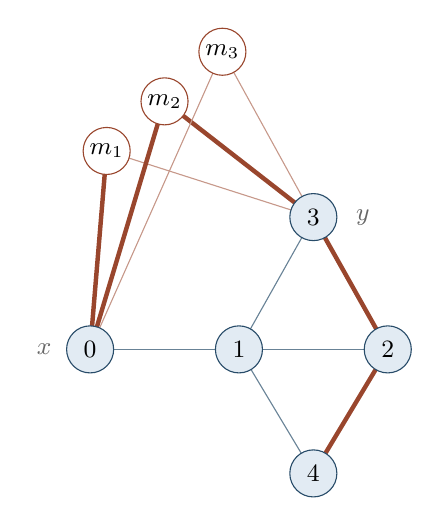
\begin{tikzpicture}[scale=1.05, every node/.style={font=\small},
  v/.style={circle, draw=inkblue, fill=softblue, inner sep=1.6pt, minimum size=17pt},
  n/.style={circle, draw=rust, fill=white, inner sep=1.2pt, minimum size=17pt}]
\draw[inkblue!70] (0.0,0.0) -- (1.8,0.0);
\draw[inkblue!70] (1.8,0.0) -- (3.6,0.0);
\draw[inkblue!70] (1.8,0.0) -- (2.7,1.6);
\draw[inkblue!70] (1.8,0.0) -- (2.7,-1.5);
\draw[rust, line width=1.6pt] (3.6,0.0) -- (2.7,1.6);
\draw[rust, line width=1.6pt] (3.6,0.0) -- (2.7,-1.5);
\draw[rust, line width=1.6pt] (0.2,2.4) -- (0.0,0.0);
\draw[rust!55] (0.2,2.4) -- (2.7,1.6);
\draw[rust, line width=1.6pt] (0.9,3.0) -- (0.0,0.0);
\draw[rust, line width=1.6pt] (0.9,3.0) -- (2.7,1.6);
\draw[rust!55] (1.6,3.6) -- (0.0,0.0);
\draw[rust!55] (1.6,3.6) -- (2.7,1.6);
\node[v] (0) at (0.0,0.0) {0};
\node[v] (1) at (1.8,0.0) {1};
\node[v] (2) at (3.6,0.0) {2};
\node[v] (4) at (2.7,-1.5) {4};
\node[v] (3) at (2.7,1.6) {3};
\node[n] (m1) at (0.2,2.4) {$m_1$};
\node[n] (m2) at (0.9,3.0) {$m_2$};
\node[n] (m3) at (1.6,3.6) {$m_3$};
\node[font=\small, text=black!60, anchor=west] at (3.1,1.6) {$y$};
\node[font=\small, text=black!60, anchor=east] at (-0.35,0) {$x$};
\end{tikzpicture}

\caption{The $6a+1$ family with $a=3$: $H$ is $K_4$ minus an edge on $\{1,2,3,4\}$ with the extra vertex
$0$, and the new vertices are joined to $x=0$ and $y=3$. The highlighted path from $4$ to $m_1$ passes the new
vertex $m_2$ as $3\,m_2\,0$; no path can pass two new vertices.}
\label{fig:family}
\end{figure}

\begin{lemma}\label{lem:line}
Fix two vertices $u\ne v$ of $G_a$. The number of simple paths between $u$ and $v$ is $A+Bt$, where $t$ is the number of
new vertices other than $u$ and $v$, and $A$, $B$ depend only on $H$ and on which vertices $u$ and $v$ are
(a vertex of $H$, or a new vertex).
\end{lemma}

\begin{proof}
A new vertex inside a path has both of its path neighbours among its own neighbours, so the path runs
$x\,m\,y$ or $y\,m\,x$ there. A simple path visits $x$ once and $y$ once, so at most one new vertex lies inside
it. The paths with no new vertex inside are paths in $H$ together with $u$ and $v$; their number $A$ does not
depend on $a$. The paths with exactly one new vertex $m$ inside correspond, for each choice of $m$, to the same
set of paths with $m$ renamed; so there are $B$ of them for each of the $t$ choices.
\end{proof}

Read as a statement about $a$: every pair of vertices of $G_a$ has a path count that is a straight line in $a$
(with $t=a$, $a-1$ or $a-2$ according as $u$ and $v$ include zero, one or two new vertices), and two values
determine the line. So $f(G_a)$ is the largest of finitely many lines, and a claim such as $f(G_a)=6a+1$ for
every $a\ge1$ reduces to checking that one line is $6a+1$ and that every other line has slope at most $6$ and
lies below $6a+1$ at the first $a$ where its pair exists. Table~\ref{tab:families} lists four choices of $H$.

\begin{table}[ht]
\centering
\begin{tabular}{llll}
\toprule
$H$ (edges) & $x,\ y$ & $f(G_a)$, every $a\ge1$ & a best pair\\
\midrule
$01,\,12$ \quad (so $G_a=K_{2,a+1}$) & $0,\ 2$ & $2a$ & $1,\ m_1$\\
$01,\,12,\,13,\,14,\,23,\,24$ & $0,\ 3$ & $6a+1$ & $4,\ m_1$\\
$01,\,02,\,03,\,04,\,05,\,12,\,23,\,25,\,34$ & $2,\ 4$ & $6a+9$ & $1,\ m_1$\\
$01,\,03,\,04,\,05,\,12,\,15,\,23,\,25,\,34$ & $0,\ 2$ & $6a+11$ & $1,\ 4$\\
\bottomrule
\end{tabular}
\caption{Four families. The counts were found and checked by computer through Lemma~\ref{lem:line}; one is
worked by hand below.}
\label{tab:families}
\end{table}

\paragraph{One line by hand.} In the $6a+1$ family (Figure~\ref{fig:family}) take $u=4$ and a new vertex
$m=m_1$. A path from $4$ to $m$ ends with the step $0\,m$ or $3\,m$.
\begin{itemize}
\item Ending $0\,m$: the path reaches $0$ either from $1$, along one of the $3$ paths $4\,1$, $4\,2\,1$,
$4\,2\,3\,1$, or from another new vertex $m'$ that it reached from $3$, along one of the $4$ paths from $4$ to
$3$ inside $\{1,2,3,4\}$. That gives $3+4(a-1)$.
\item Ending $3\,m$: the path reaches $3$ either inside $\{1,2,3,4\}$, in $4$ ways, or as $1\,0\,m'\,3$ after
one of the $2$ paths from $4$ to $1$ that avoid $3$. That gives $4+2(a-1)$.
\end{itemize}
The total is $6a+1$. Lemma~\ref{lem:line} and the finite check show that no other pair does better.

\paragraph{Proof of Theorem~\ref{thm:main}.} The family $2a$ gives every even number. Every odd number from
$15$ on is $6a+1$, $6a+9$ or $6a+11$ with $a\ge1$, according to its residue modulo $6$, and the $6a+1$ family
also gives $7$ and $13$. That leaves $1$, $5$, $9$ and $11$: $f(K_2)=1$, $f(K_4)=5$, $f(W_4)=9$ for the wheel
with four rim vertices (two opposite rim vertices), and $f=11$ for the graph with edges $01$, $02$, $05$,
$12$, $13$, $14$, $15$, $34$, $45$ (between $2$ and $3$). $\square$

\section{Why three is impossible}

\begin{proposition}\label{prop:three}
No graph has $f(G)=3$.
\end{proposition}

\begin{proof}
A path between $u$ and $v$ passes through the same blocks (maximal $2$-connected pieces and bridges) in the
same order, entering and leaving each at fixed cut vertices, so the number of paths between $u$ and $v$ is the product of
the numbers of paths inside those blocks. A bridge contributes $1$ and a cycle $2$. If some pair has exactly
$3$ paths, then $3$ is prime, so one block $B$ has a pair with $3$ paths; $B$ is $2$-connected and not a cycle.
Such a graph contains a theta graph: three internally disjoint paths between two vertices. In a graph without
multiple edges at most one of the three is a single edge, so two of them have interior vertices $s$ and $t$. A
path from $s$ leaves along its own branch towards one of the two ends, then reaches $t$ either directly along
$t$'s branch or round the third branch and back; that is $2\times2=4$ paths inside the theta alone. So
$f(G)\ge4$.
\end{proof}

\begin{remark}\label{rem:glue}
Gluing two graphs at a vertex that is an end of a best pair in each multiplies $f$: a path between the two sides
crosses the shared vertex once, and no pair on one side gains paths. With this, any $k=k_1k_2$ is realised once
$k_1$ and $k_2$ are. A computer search over all connected $H$ with at most seven vertices found no family of slope $2$
with odd values, and none of slope $4$ with values $1 \bmod 4$; that is why the odd families have slope $6$.
\end{remark}

\paragraph{Verification.} Lemma~\ref{lem:line} and the four families are checked in Lean~4 with
Mathlib~\cite{mathlib}, with paths as lists of distinct vertices. The proof follows the text: a generator of
all simple paths is proved exact, paths transfer between $G_b$ and $G_a$ along embeddings, a path has at most
one interior new vertex, and the count in $G_a$ is $N_b+(a-b)T$ for an embedded copy of a small $G_b$. The
finitely many lines and the small graphs are then checked by evaluation. The final theorem states
Theorem~\ref{thm:main} for simple graphs, using only the standard axioms. Proposition~\ref{prop:three} is
proved here by hand and not formalised. A plain Python program, independent of the Lean code, recomputes every
line. Everything is at \url{https://github.com/jvvk/mathematics/tree/main/every-path-count-but-three}.

\paragraph{Acknowledgements.} The question was asked by Mikhail Tikhomirov on MathOverflow; the comment there by
Joseph Gordon suggested gluing complete bipartite graphs. Anthropic's Claude (Opus~5.5)
was used to find the families, write the programs and the Lean formalisation, and draft this text. The author
takes responsibility for the content.

\begin{thebibliography}{9}
\bibitem{IOI} International Olympiad in Informatics 2020, Day 1, task ``Connecting Supertrees''
(\texttt{supertrees}), \url{https://ioinformatics.org/files/ioi2020problem2.pdf}, accessed 11 October 2026.
\bibitem{MO} M.~Tikhomirov, Largest number of simple paths between two vertices, MathOverflow question 371851
(16 September 2020),
\url{https://mathoverflow.net/q/371851}, accessed 11 October 2026.
\bibitem{mathlib} The mathlib Community, The Lean mathematical library, in \emph{Proceedings of the 9th ACM
SIGPLAN International Conference on Certified Programs and Proofs (CPP 2020)}, 367--381,
\href{https://doi.org/10.1145/3372885.3373824}{doi:10.1145/3372885.3373824}.
\end{thebibliography}

\bigskip
\noindent Vamshi Jandhyala, London, UK.

\end{document}
